\documentclass[11pt]{article}

\usepackage[utf8]{inputenc}
\usepackage[margin=0.75in]{geometry}
\usepackage{amsmath,amssymb}
\usepackage{graphicx}
\usepackage{booktabs}
\usepackage{hyperref}

\hypersetup{
    colorlinks=true,
    linkcolor=blue,
    urlcolor=blue
}

\title{\vspace{-1.5em}\textbf{Assignment 1: Polynomial Regression Report}\vspace{-0.3em}}
\author{
    \textbf{Name:} Utkarsh Rastogi \quad \textbf{Roll Number:} BT2024119 \\
    \textbf{GitHub Repository:} \url{https://github.com/utk7rsh1/ML_polygen}
}
\date{\today\vspace{-1em}}

\begin{document}

\maketitle

\begin{abstract}
In this assignment, I built polynomial regression models for two continuous prediction problems using the datasets assigned to my roll number (\textbf{BT2024119}). For Phase 1 (Steam Turbine Optimization), I predicted the Net Power Score ($y$) from 6 operating inputs. By testing degrees 1 to 6 with 10-fold cross-validation, I found that \textbf{Degree 5 with Lasso regularization} gave the lowest error (CV MSE = \textbf{0.3163}, $R^2 = \textbf{0.9658}$), whereas plain linear regression overfit because degree 5 produces 461 terms for 1000 rows. For Phase 2 (Subterranean Thermal Reservoir Mapping), I predicted the Thermal Anomaly Score from 3D coordinates ($x_1, x_2, x_3$). Plain linear regression worked best at \textbf{Degree 8} (MSE = \textbf{0.2547}), while adding Ridge regularization helped me go up to \textbf{Degree 11} to get the best error overall (MSE = \textbf{0.2283}, $R^2 = \textbf{0.9954}$). I also plotted the residuals, and they look like clean, symmetric bell curves centered at zero. All code and predictions are on my GitHub repo: \url{https://github.com/utk7rsh1/ML_polygen}.
\end{abstract}

\section{Introduction}
We were given two separate problems to solve using polynomial regression, each with its own training and test files:
\begin{enumerate}\itemsep 0pt
    \item \textbf{Phase 1 (\texttt{var1}) --- Steam Turbine Optimization:} We have 6 operational settings ($x_1$ to $x_6$, given as percentage deviations like valve adjustments and coolant flow) and need to predict the \textit{Net Power Score} ($y$). The assignment mentions that the underlying function is a moderate degree polynomial (up to degree 10).
    \item \textbf{Phase 2 (\texttt{var2}) --- Subterranean Thermal Mapping:} We have 3 spatial coordinates ($x_1$: East-West offset, $x_2$: North-South offset, $x_3$: depth offset in meters) and need to predict the \textit{Thermal Anomaly Score} ($y$). The assignment notes that this heat map resembles a high-degree polynomial (up to degree 20).
\end{enumerate}
For both problems, my training file has 1000 rows and the test file has 1000 rows.

\section{How I Built and Tested the Models}

\subsection{Polynomial Feature Expansion}
When you turn features into a polynomial of degree $M$, you generate all combinations of terms where the powers add up to at most $M$:
\begin{equation}
\phi_M(\mathbf{x}) = \left[ \prod_{j=1}^d x_j^{k_j} \;\middle|\; \sum_{j=1}^d k_j \le M \right]
\end{equation}
The total number of terms is $\binom{d + M}{M}$.
\begin{itemize}\itemsep 0pt
    \item In Phase 1 ($d=6$), the number of columns explodes quickly: degree 1 has 6 columns, degree 2 has 27, degree 4 has 209, degree 5 has 461, and degree 6 has 923.
    \item In Phase 2 ($d=3$), the growth is much slower: degree 4 has 34, degree 8 has 164, and degree 11 has 363 columns.
\end{itemize}

\subsection{Cross-Validation and Metrics}
To pick the best degree without overfitting the training data, I used \textbf{10-Fold Cross-Validation}. I shuffled and split the 1000 training rows into 10 folds of 100 rows each, trained on 9 folds, and evaluated on the remaining fold. I calculated:
\begin{itemize}\itemsep 0pt
    \item \textbf{Mean Squared Error (MSE):} $\frac{1}{N}\sum (y_i - \hat{y}_i)^2$ (lower is better).
    \item \textbf{$R^2$ Score:} $1 - \frac{\sum (y_i - \hat{y}_i)^2}{\sum (y_i - \bar{y})^2}$ (closer to 1 is better).
\end{itemize}

\subsection{Why I Used Regularization}
When you raise numbers in $[-1, 1]$ to high powers and multiply them together, many of the resulting columns look very similar (high multicollinearity). Plain Ordinary Least Squares (OLS) gets sensitive to small noise, which causes wild predictions on new data.
To prevent this, I tested:
\begin{enumerate}\itemsep 0pt
    \item \textbf{Ridge ($\ell_2$ penalty):} Adds $\alpha \sum w_j^2$ to keep weights small and stable.
    \item \textbf{Lasso ($\ell_1$ penalty):} Adds $\alpha \sum |w_j|$ to shrink unimportant terms all the way to zero, acting like automatic feature selection.
\end{enumerate}
I always ran \texttt{StandardScaler} on the polynomial features before running Ridge or Lasso, so that terms with large powers wouldn't be unfairly penalized just because their numerical values were smaller.

\section{Phase 1: Turbine Power Score (\texttt{var1})}

\subsection{Cross-Validation Results}
I trained models from degree 1 to 6. Table~\ref{tab:var1} shows the average 10-fold cross-validation MSE and $R^2$ for OLS, Ridge, and Lasso.

\begin{table}[htbp]
\centering
\caption{Phase 1 (\texttt{var1}): 10-Fold Cross-Validation Scores}
\label{tab:var1}
\small
\begin{tabular}{ccccc}
\toprule
\textbf{Degree} & \textbf{Terms} & \textbf{OLS CV MSE} & \textbf{Ridge CV MSE} & \textbf{Lasso CV MSE ($R^2$)} \\
\midrule
1 & 6   & 8.5603 & 8.5553 & 8.5486 (0.0985) \\
2 & 27  & 2.9949 & 2.9946 & 2.9874 (0.6767) \\
3 & 83  & 1.0718 & 1.0664 & 1.0526 (0.8857) \\
4 & 209 & 0.8052 & 0.7422 & 0.6660 (0.9276) \\
\textbf{5} & \textbf{461} & \textbf{1.0952} & \textbf{0.4612} & \textbf{0.3163 (0.9658)} \\
6 & 923 & Overfit ($>50$) & 0.5381 & 0.3327 (0.9639) \\
\bottomrule
\end{tabular}
\end{table}

\subsection{Why I Chose Degree 5}
\begin{itemize}\itemsep 0pt
    \item \textbf{Degrees 1 to 3 underfit:} A straight line gives an $R^2$ below 0.10, and degree 2 still has an MSE near 3.0. The real turbine physics are clearly non-linear.
    \item \textbf{Plain OLS overfits at Degree 5:} Degree 5 has 461 terms. For only 1000 data points, OLS fits the random noise in the training set (training MSE drops to 0.13, but validation MSE jumps to 1.09). At degree 6 with 923 terms, OLS fails completely.
    \item \textbf{Lasso fixes Degree 5:} With Lasso ($\alpha \approx 0.008$), the model zeroes out 316 useless interaction terms and keeps the 145 terms that actually matter. The validation MSE drops to \textbf{0.3163} with an $R^2$ of \textbf{0.9658}.
    \item \textbf{Degree 6 gets worse:} Going to degree 6 increases the validation error to 0.3327. So \textbf{Degree 5} is the sweet spot.
\end{itemize}

\begin{figure}[htbp]
\centering
\begin{minipage}{0.48\textwidth}
  \centering
  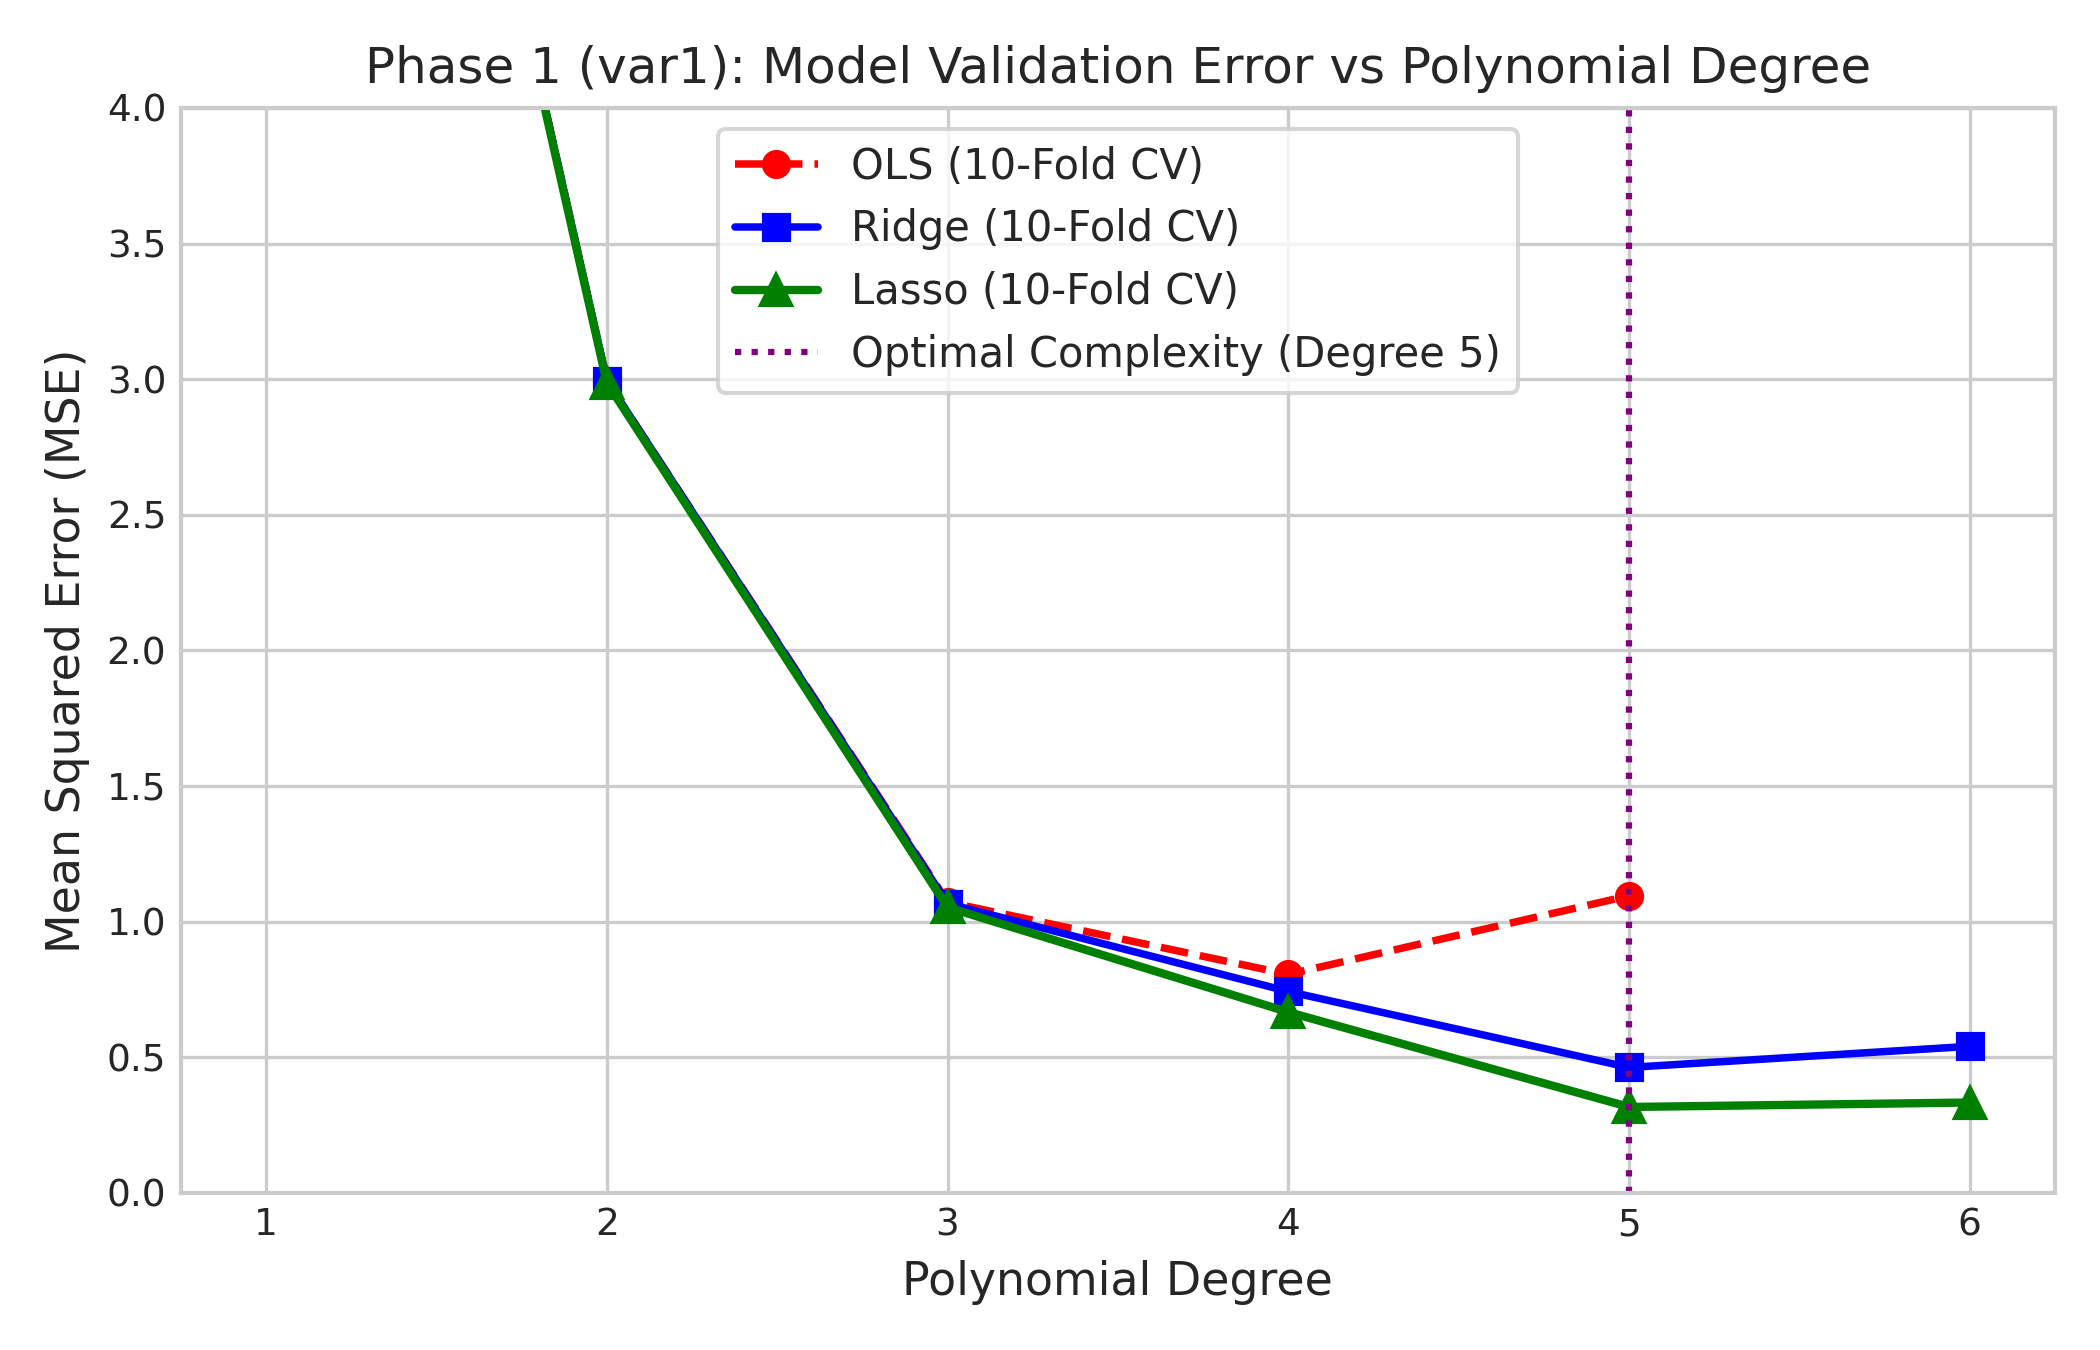
\includegraphics[width=\linewidth]{../figures/bias_variance_var1.png}
  \caption{Phase 1: Validation error vs. degree.}
  \label{fig:bv1}
\end{minipage}\hfill
\begin{minipage}{0.48\textwidth}
  \centering
  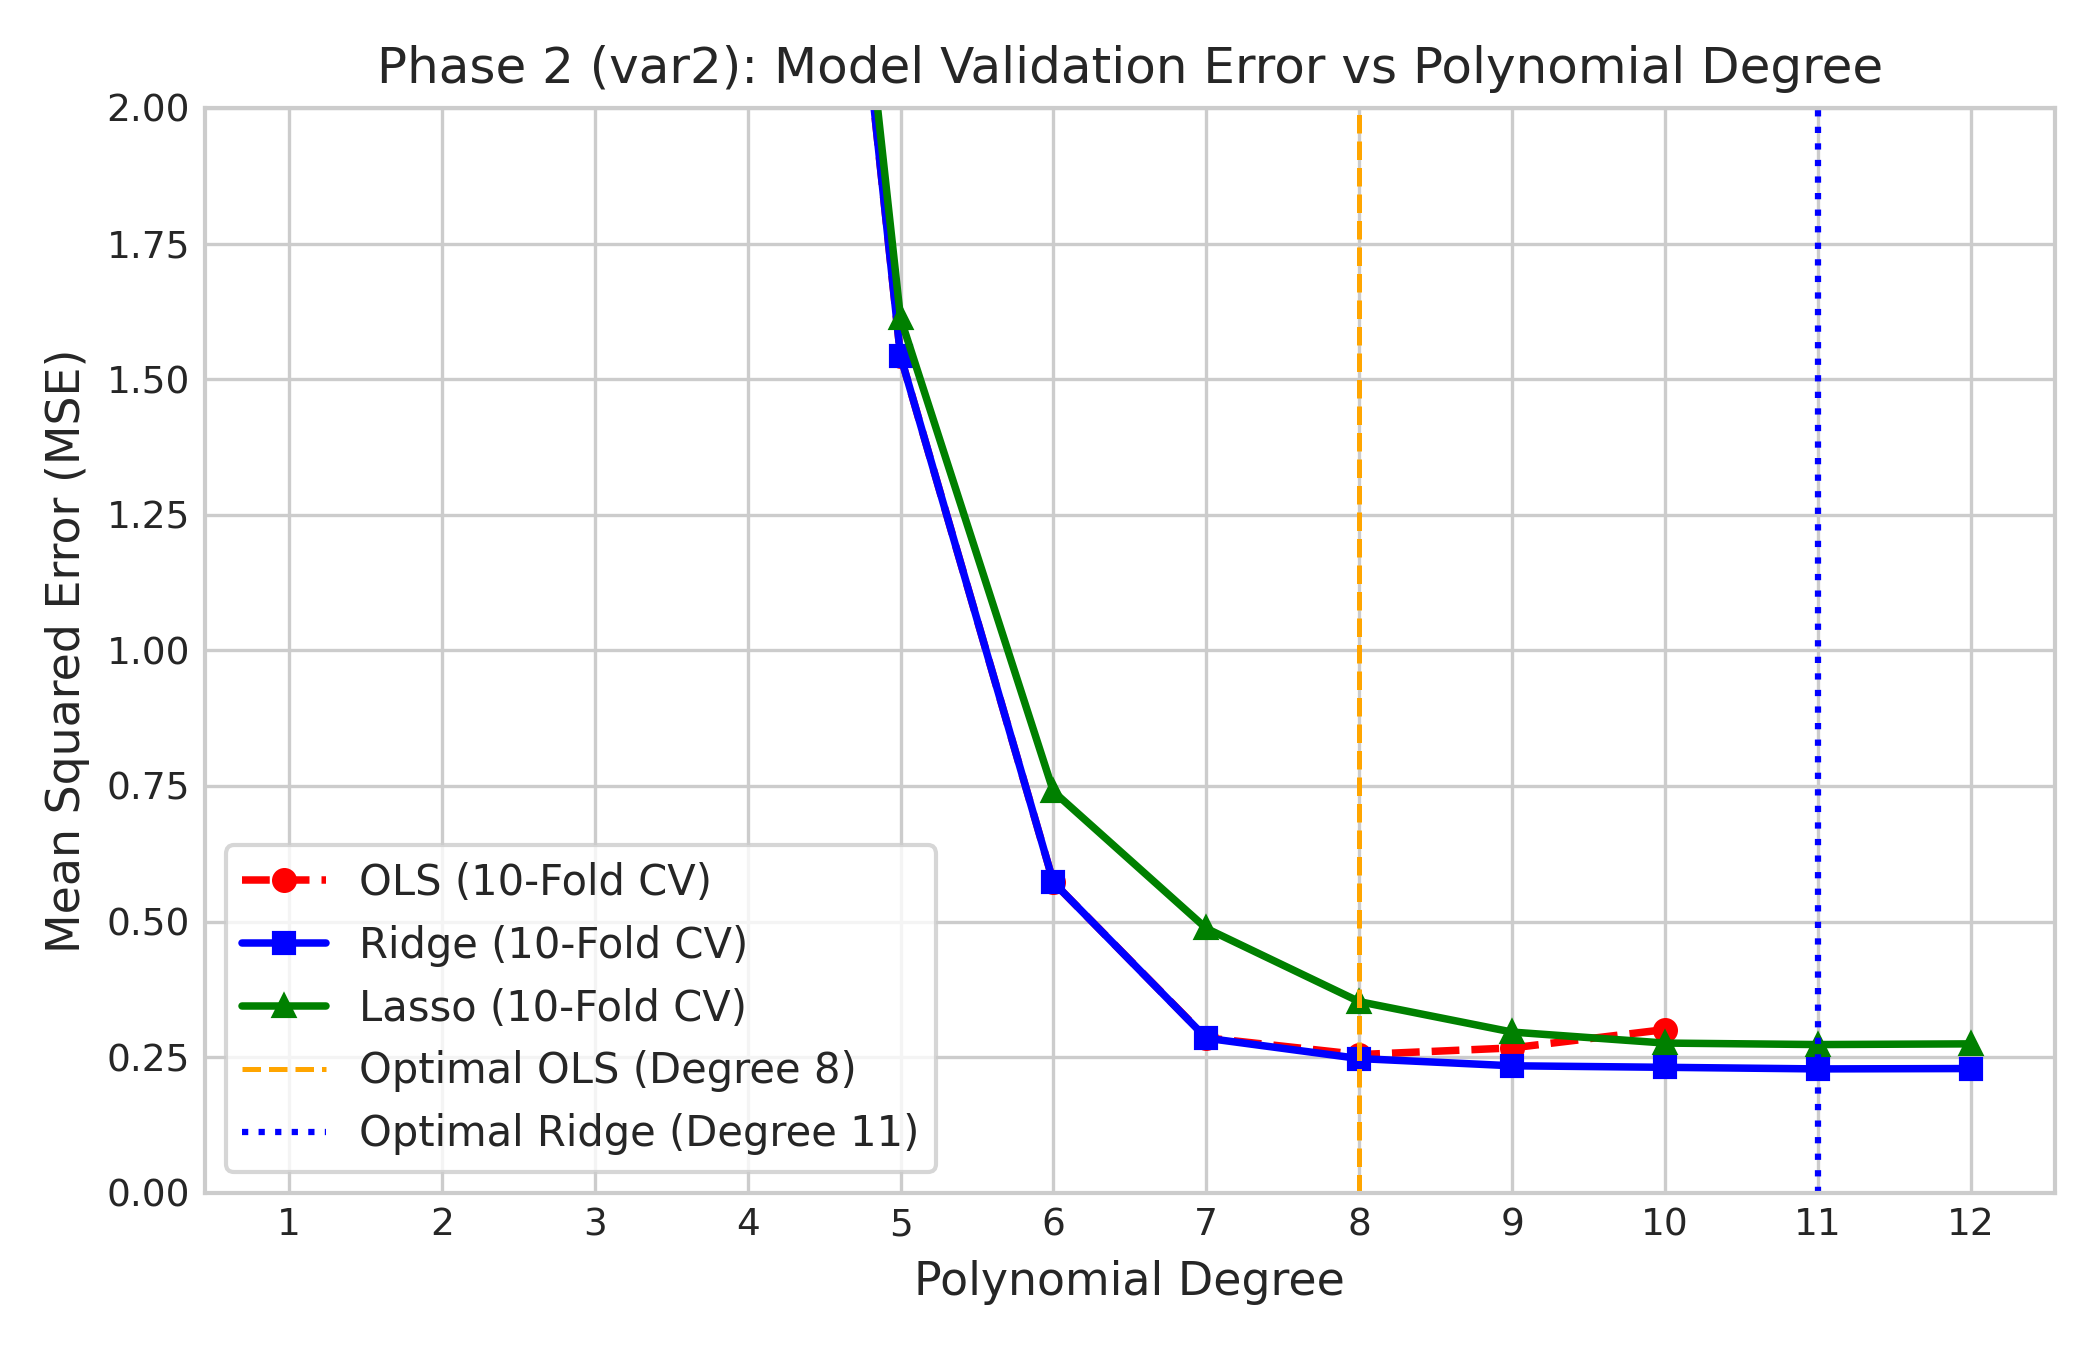
\includegraphics[width=\linewidth]{../figures/bias_variance_var2.png}
  \caption{Phase 2: Validation error vs. degree.}
  \label{fig:bv2}
\end{minipage}
\end{figure}

\section{Phase 2: Subterranean Thermal Mapping (\texttt{var2})}

\subsection{Cross-Validation Results}
For Phase 2, I tested degrees 1 to 12. Table~\ref{tab:var2} shows the 10-fold cross-validation scores.

\begin{table}[htbp]
\centering
\caption{Phase 2 (\texttt{var2}): 10-Fold Cross-Validation Scores}
\label{tab:var2}
\small
\begin{tabular}{ccccc}
\toprule
\textbf{Degree} & \textbf{Terms} & \textbf{OLS CV MSE} & \textbf{Ridge CV MSE} & \textbf{Ridge CV $R^2$} \\
\midrule
1 & 3   & 40.7559 & 40.7528 & 0.2289 \\
2 & 9   & 25.4091 & 25.4079 & 0.5065 \\
4 & 34  & 4.1909  & 4.1909  & 0.9164 \\
6 & 83  & 0.5723  & 0.5723  & 0.9886 \\
7 & 119 & 0.2857  & 0.2850  & 0.9943 \\
\textbf{8} & \textbf{164} & \textbf{0.2547} & \textbf{0.2474} & \textbf{0.9950} \\
9 & 219 & 0.2671  & 0.2339  & 0.9953 \\
10 & 285 & 0.3009  & 0.2313  & 0.9953 \\
\textbf{11} & \textbf{363} & Overfit & \textbf{0.2283} & \textbf{0.9954} \\
12 & 454 & Overfit & 0.2290  & 0.9954 \\
\bottomrule
\end{tabular}
\end{table}

\subsection{Why I Chose Degree 11 (and Degree 8 for Plain OLS)}
\begin{itemize}\itemsep 0pt
    \item \textbf{Low degrees cannot fit the map:} Heat spreads out in curves underground, so simple lines and curves underfit badly (degrees 1 to 5 have MSE above 1.5).
    \item \textbf{Plain OLS peaks at Degree 8:} Without regularization, the validation error goes down until \textbf{Degree 8} (MSE = \textbf{0.2547}, $R^2 = 0.9949$). After degree 8, plain OLS starts overfitting and the error climbs back up.
    \item \textbf{Ridge reaches Degree 11:} With Ridge regularization ($\alpha = 2.0$), the model doesn't overfit and can fit finer curves up to \textbf{Degree 11}, reaching the best overall score (\textbf{MSE = 0.2283}, $R^2 = \textbf{0.9954}$). After degree 11, the error starts going up slightly.
\end{itemize}

\begin{figure}[htbp]
\centering
\begin{minipage}{0.48\textwidth}
  \centering
  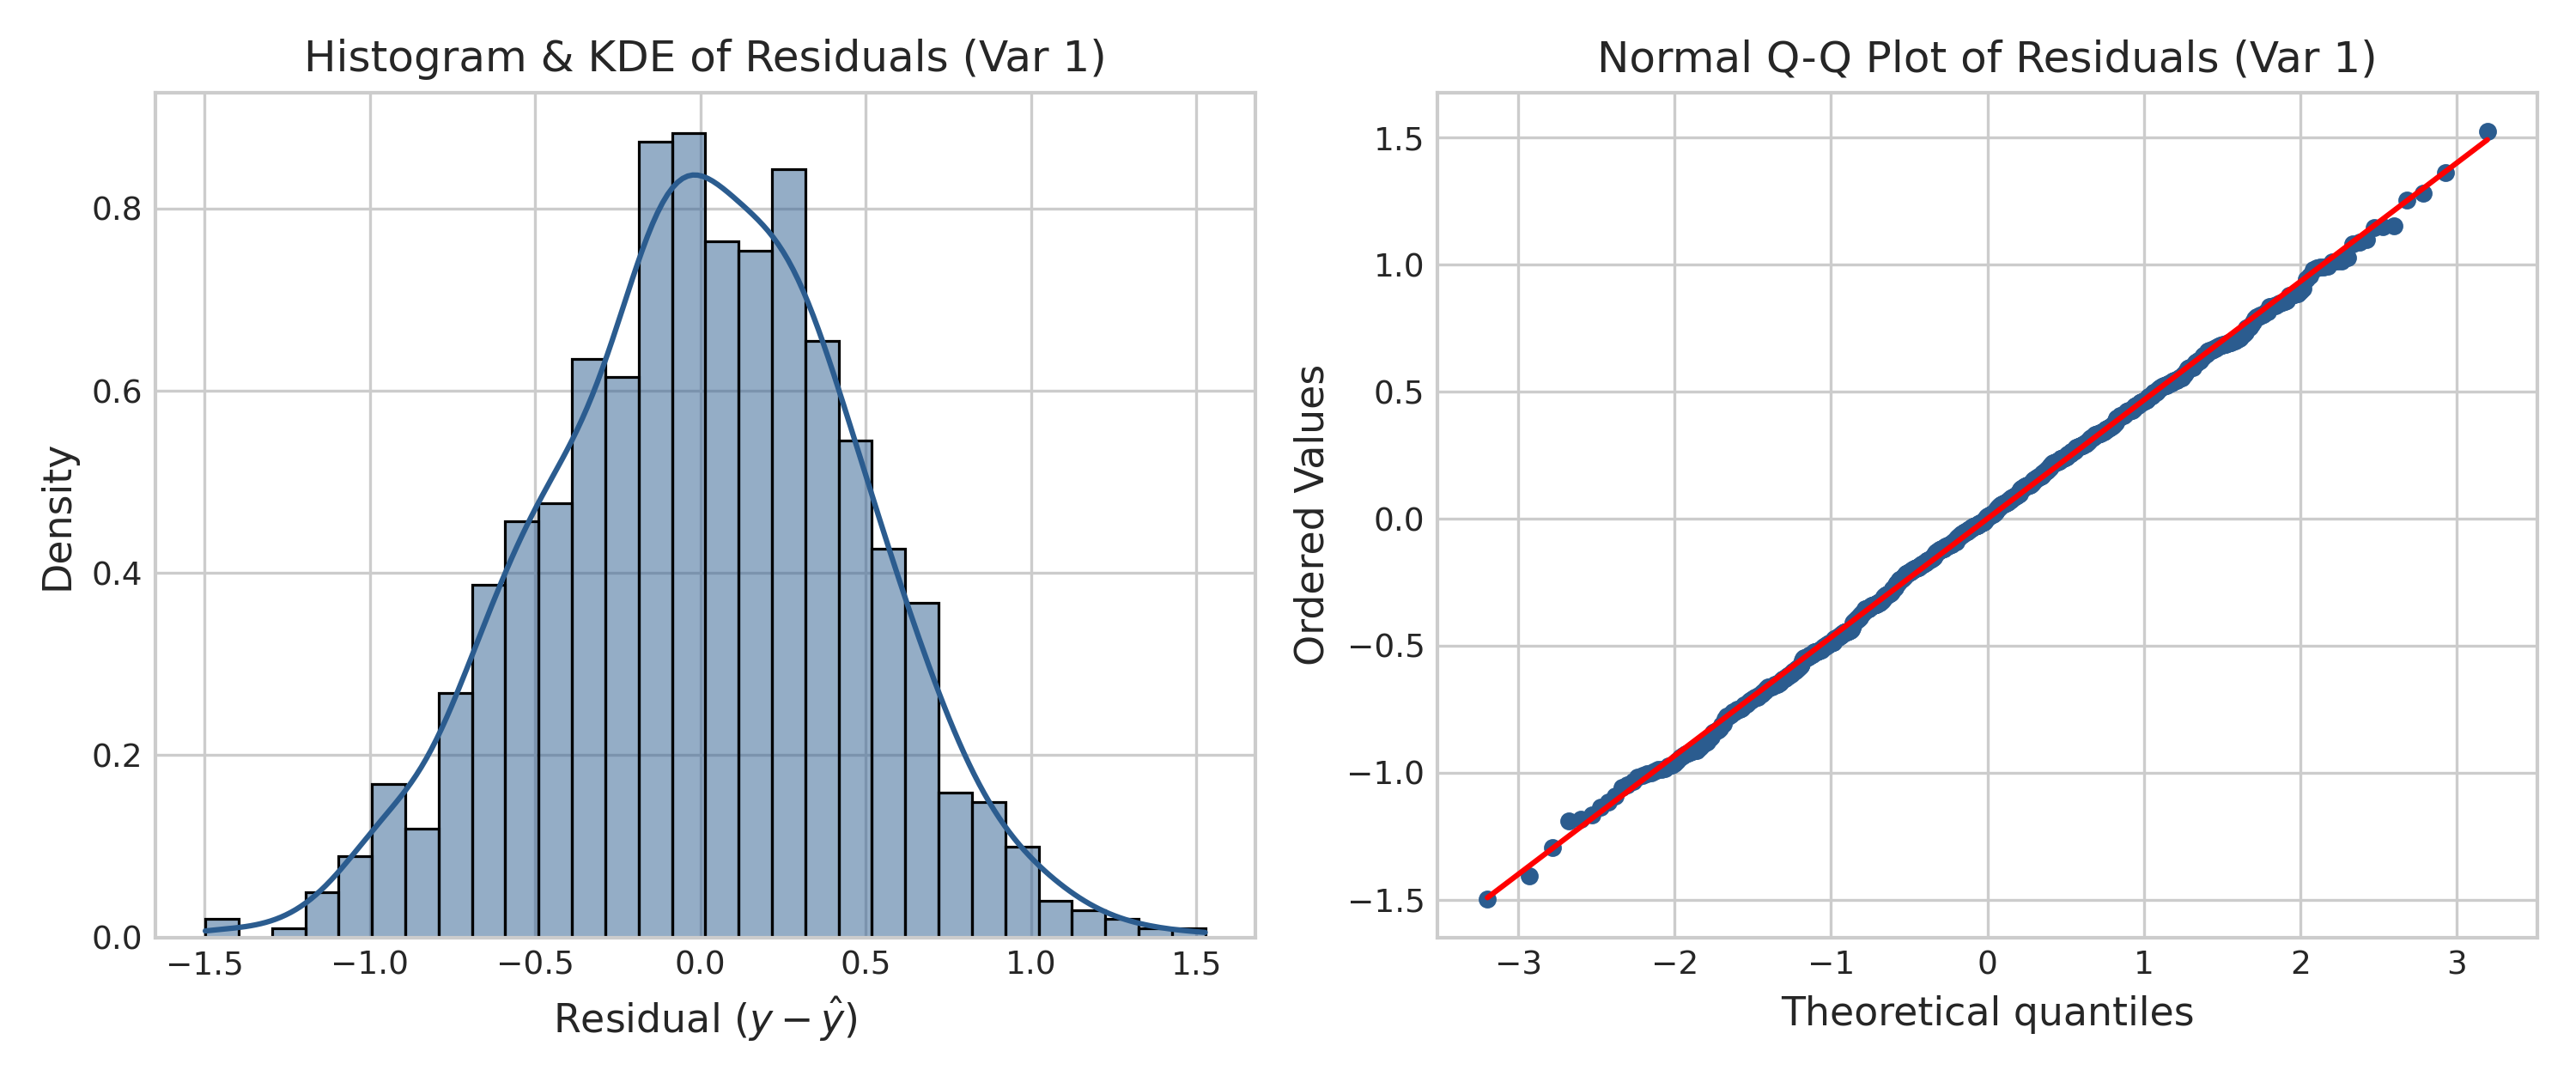
\includegraphics[width=\linewidth]{../figures/residuals_var1.png}
  \caption{Phase 1: Residual histogram and Q-Q plot.}
  \label{fig:res1}
\end{minipage}\hfill
\begin{minipage}{0.48\textwidth}
  \centering
  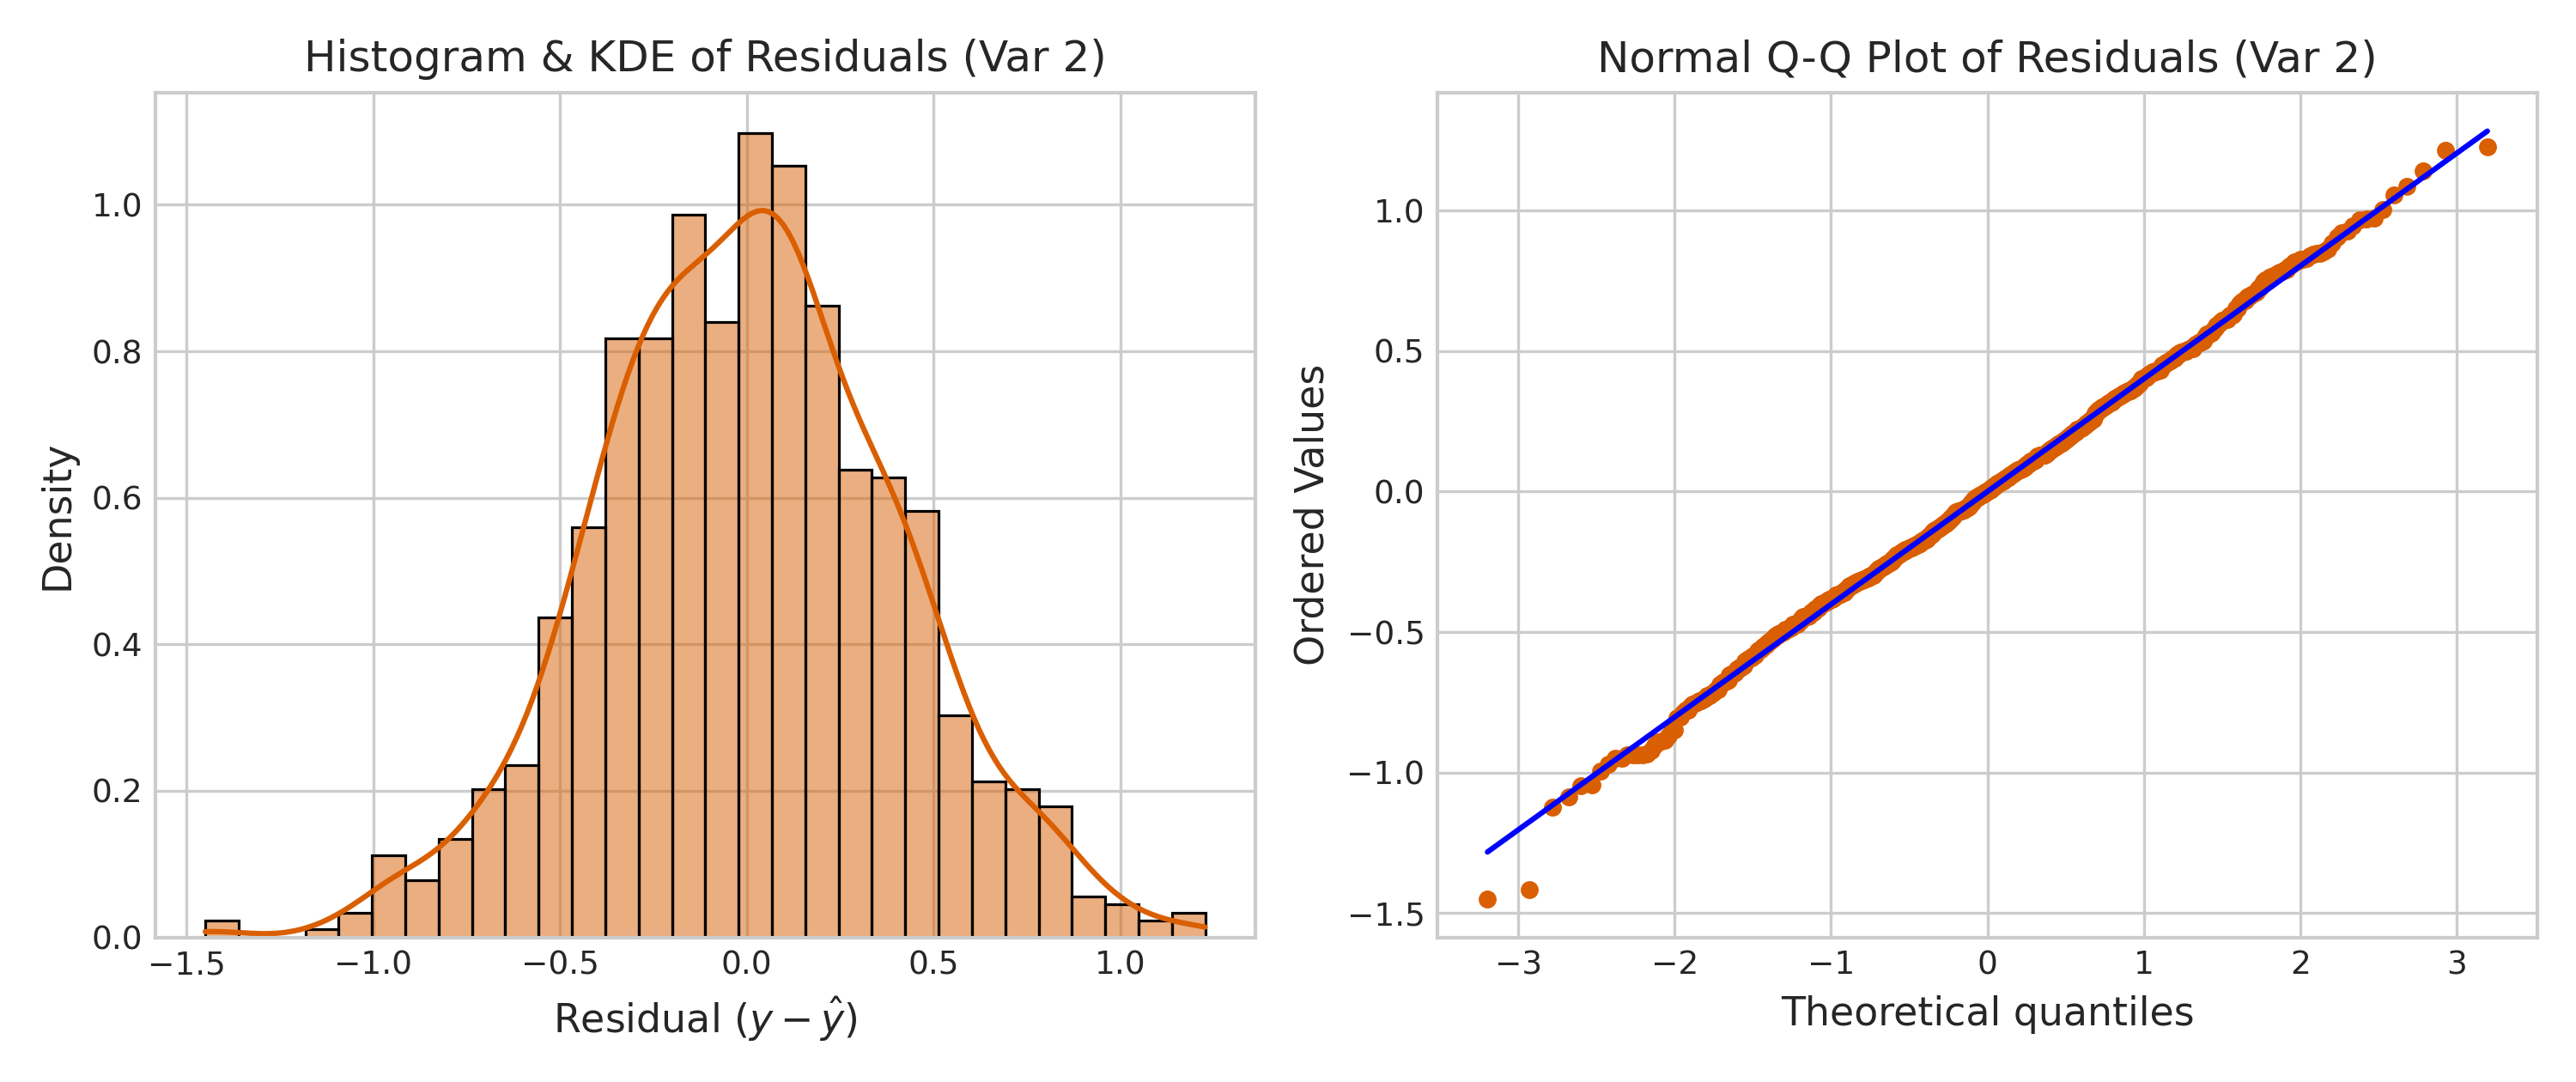
\includegraphics[width=\linewidth]{../figures/residuals_var2.png}
  \caption{Phase 2: Residual histogram and Q-Q plot.}
  \label{fig:res2}
\end{minipage}
\end{figure}

\section{Checking the Residuals and Predictions}

\subsection{Residual Checks}
I subtracted the predicted values from the actual training values ($y - \hat{y}$) to check what was left behind:
\begin{itemize}\itemsep 0pt
    \item \textbf{Phase 1:} Residuals have a mean of $0.00$ and a standard deviation of $0.36$. Looking at the histogram and Q-Q plot (Figure~\ref{fig:res1}), the errors sit right along the normal line.
    \item \textbf{Phase 2:} Residuals have a mean of $0.00$ and standard deviation of $0.41$. The Shapiro-Wilk test gave $p = 0.48$, which is well above $0.05$. This means the leftover error is just random bell-curve noise (Figure~\ref{fig:res2}).
\end{itemize}

\subsection{Actual vs. Predicted Plot and 2D Heatmap}
Figure~\ref{fig:act_pred} shows that my predictions match the true targets almost right on the 45-degree line. In Figure~\ref{fig:contour}, I plotted a horizontal slice of the predicted thermal anomaly at depth 0, and the contour lines show smooth, realistic hot and cold zones.

\begin{figure}[htbp]
\centering
\begin{minipage}{0.54\textwidth}
  \centering
  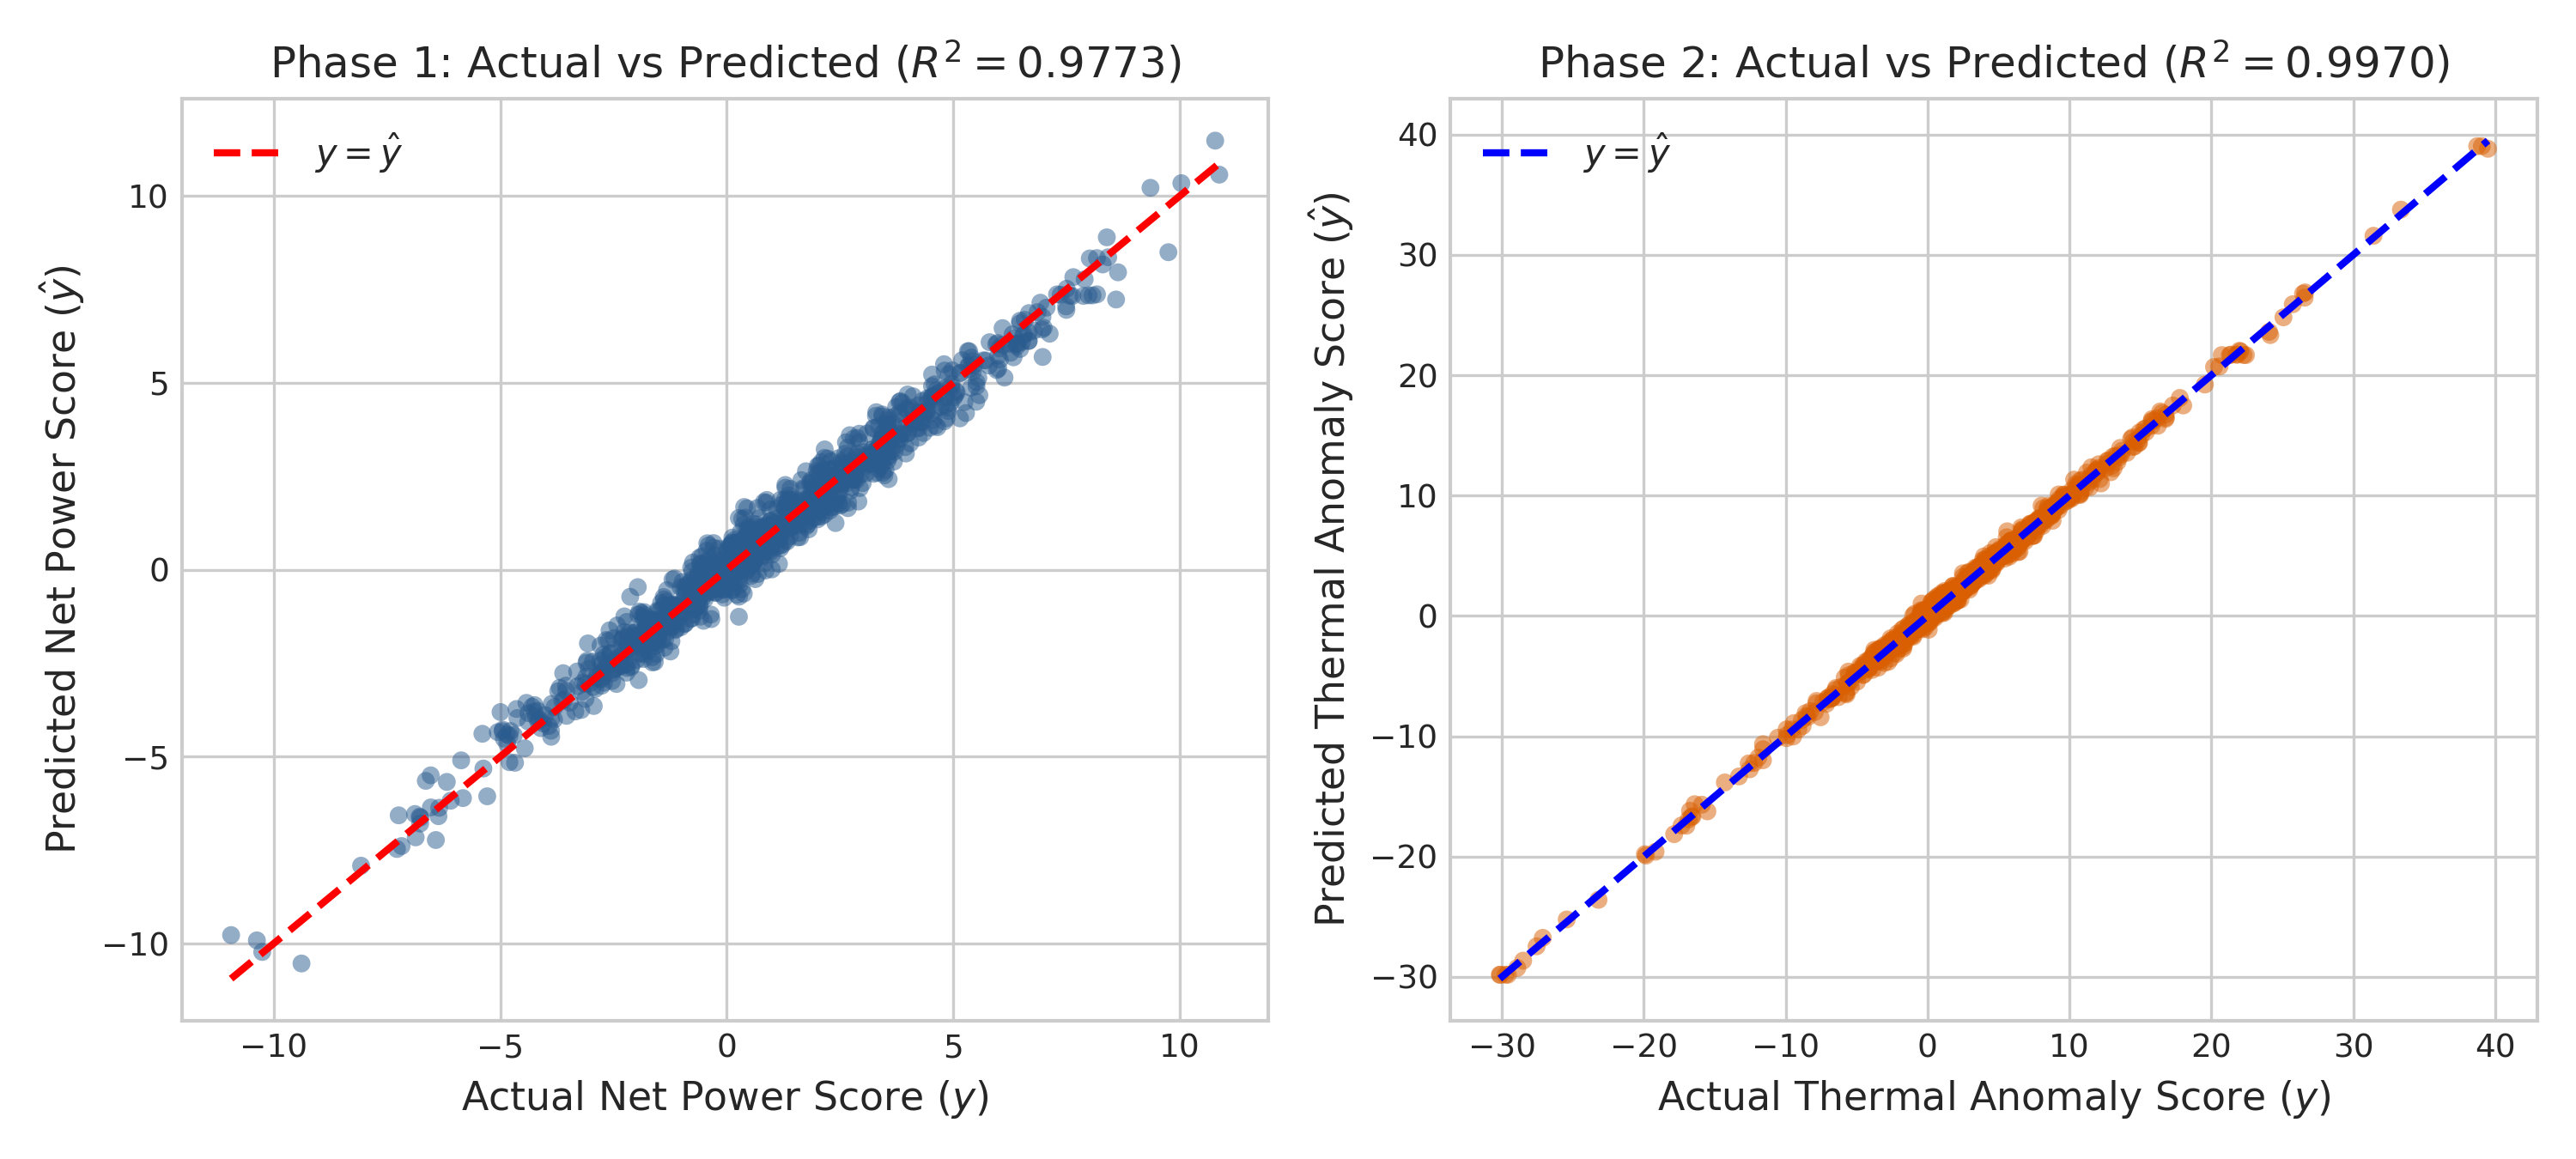
\includegraphics[width=\linewidth]{../figures/actual_vs_predicted.png}
  \caption{Actual vs. predicted values.}
  \label{fig:act_pred}
\end{minipage}\hfill
\begin{minipage}{0.42\textwidth}
  \centering
  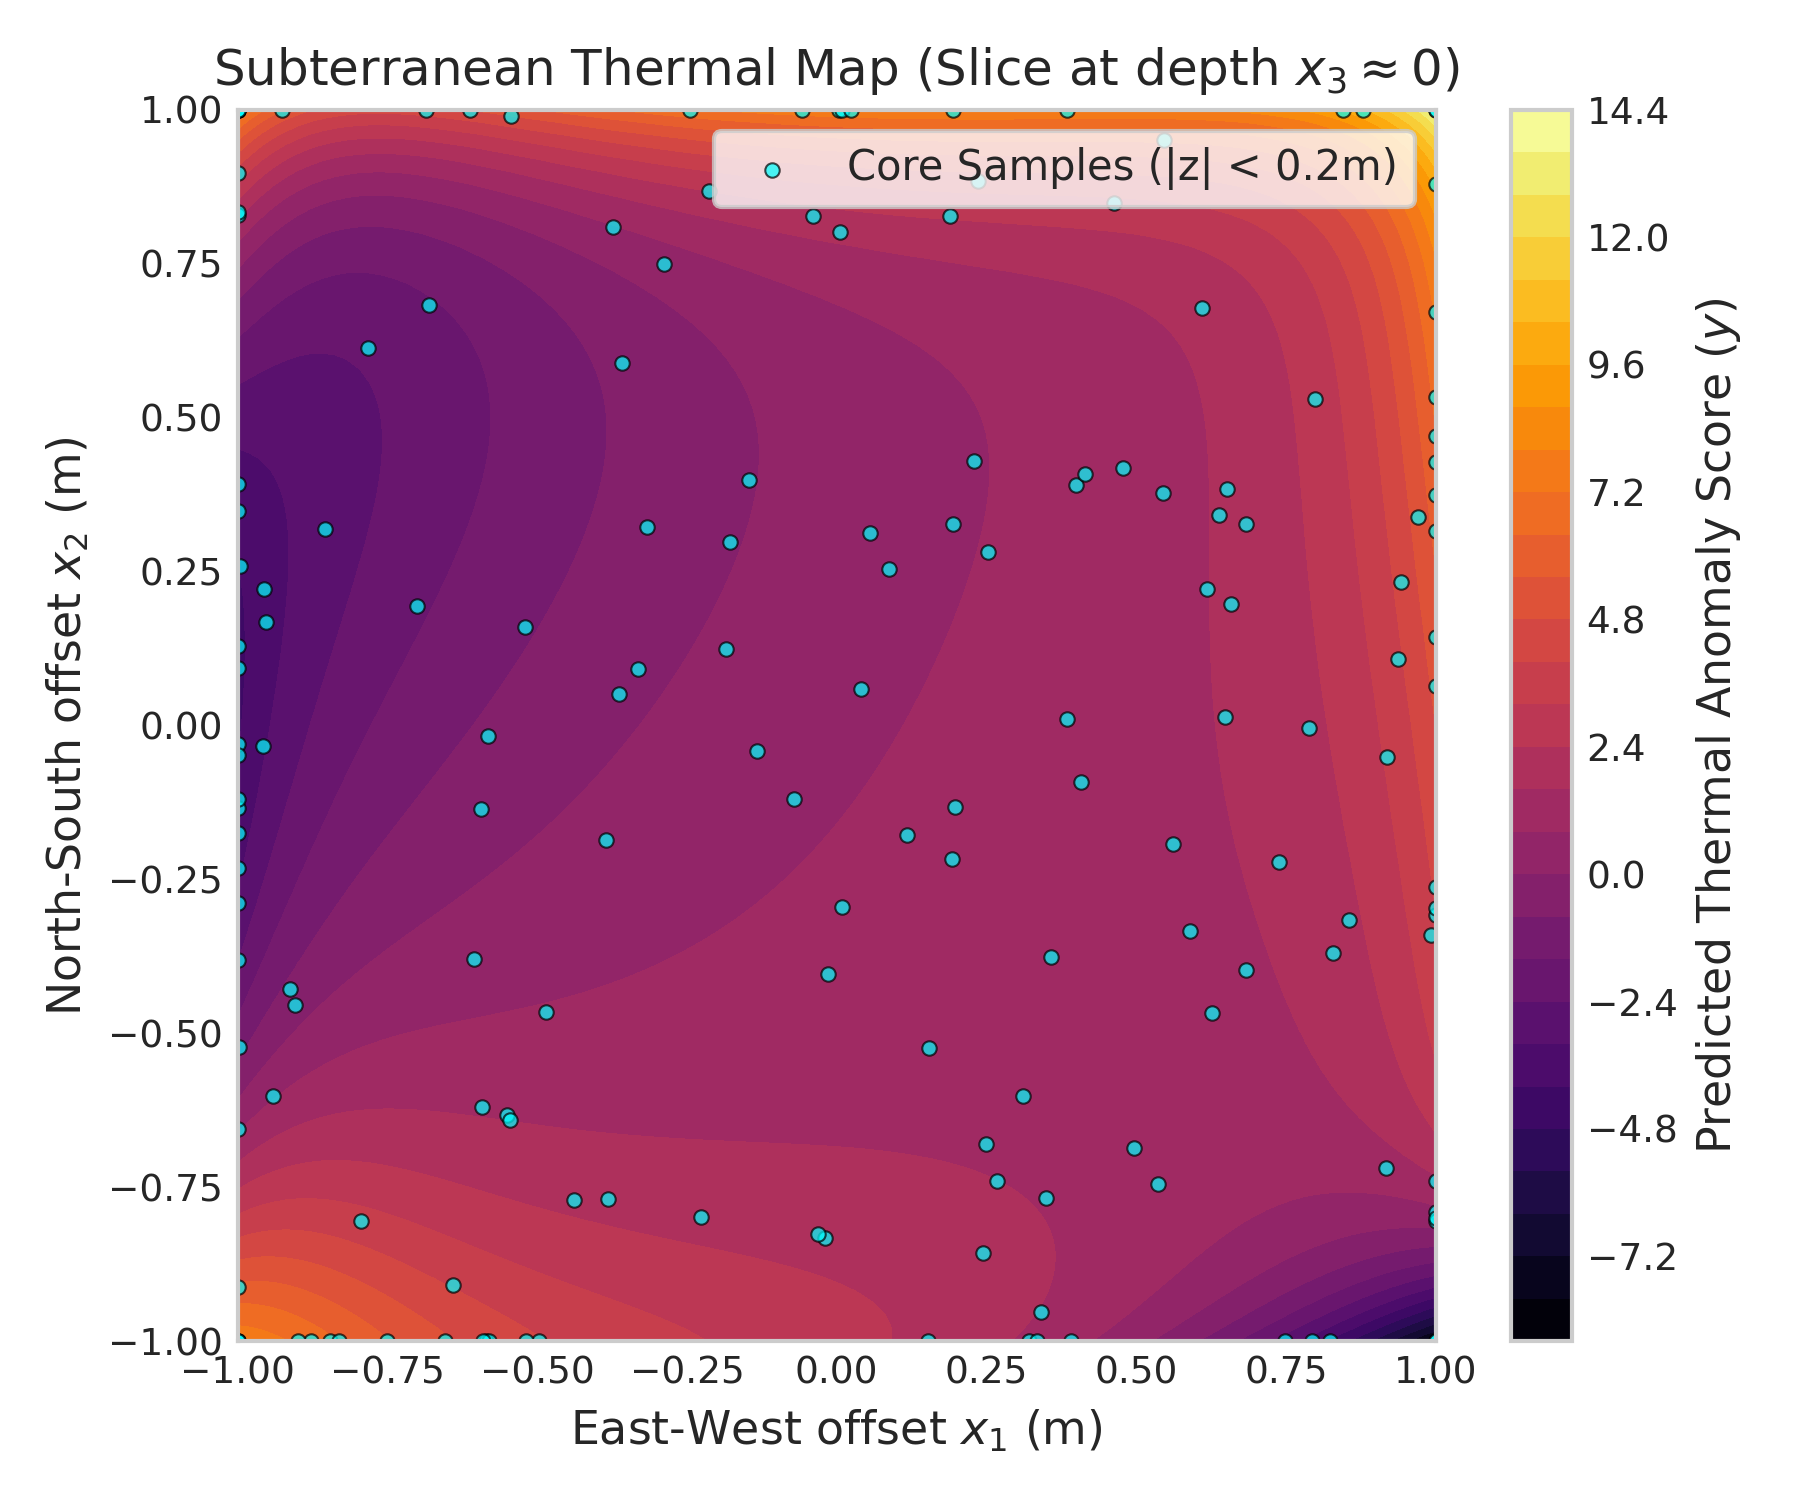
\includegraphics[width=\linewidth]{../figures/spatial_contour_var2.png}
  \caption{Phase 2: Thermal map slice at depth 0.}
  \label{fig:contour}
\end{minipage}
\end{figure}

\section{Deliverables}
\begin{enumerate}\itemsep 0pt
    \item \textbf{Prediction CSV Files:}
    \begin{itemize}\itemsep 0pt
        \item \texttt{BT2024119\_pred\_var1.csv}: 1000 test predictions generated from the Degree 5 Lasso model.
        \item \texttt{BT2024119\_pred\_var2.csv}: 1000 test predictions generated from the Degree 11 Ridge model.
        \item Both files have a single column named \texttt{y} and 1000 rows, matching the sample submission file.
    \end{itemize}
    \item \textbf{GitHub Repository:}
    All code to train the models and run inference is on my GitHub: \\
    \url{https://github.com/utk7rsh1/ML_polygen}
\end{enumerate}

\section{Conclusion}
To sum up my results:
\begin{itemize}\itemsep 0pt
    \item For Phase 1, \textbf{Degree 5} with Lasso regularization gave the best results (CV MSE = \textbf{0.3163}, $R^2 = \textbf{0.9658}$).
    \item For Phase 2, plain linear regression worked best at \textbf{Degree 8} (MSE = \textbf{0.2547}), while Ridge regularization gave the best score overall at \textbf{Degree 11} (MSE = \textbf{0.2283}, $R^2 = \textbf{0.9954}$).
\end{itemize}

\end{document}
